\chapter{Example Chapter using Formulas, Tables and Figures} 
\label{cha:derivation}

\section{Table reference}
\label{sec:features}
This is a table reference:
\tabref{tab:params} summarizes the parameters taken into account.
\begin{table}
	\caption{Considered input and target parameters.}
	\label{tab:params}
	\centering
	\begin{tabular}{l c c}
		\toprule
		parameter name & symbol & model position \\
		\midrule
		ambient temperature & $\vartheta_\mathrm{a}$ & input \\
		liquid coolant temperature & $\vartheta_\mathrm{c}$ & input \\
		actual voltage $d$-axis component & $u_\mathrm{d}$ & input \\
		actual voltage $q$-axis component & $u_\mathrm{q}$ & input \\
		actual current $d$-axis component & $i_\mathrm{d}$ & input \\
		actual current $q$-axis component & $i_\mathrm{q}$ & input \\
		\hline
		permanent magnet temperature & $\vartheta_{\mathrm{PM}}$ & output \\
		stator teeth temperature & $\vartheta_{\mathrm{ST}}$ & output \\
		stator winding temperature & $\vartheta_{\mathrm{SW}}$ & output \\
		stator yoke temperature & $\vartheta_{\mathrm{SY}}$ & output\\
		\bottomrule
	 \end{tabular}
\end{table}


\section{Formulas}
\label{subsec:normalization}
This is a in-text formula example. Note that the formulas are integrated in the text (full-stop after formula).

Note: Using variables, the variable itself should be in italic letters, the subscript should be in normal letters. Space between count and unit! Make use of 'mathrm' and 'SI'. Example $V_\mathrm{DC} = \SI{100}{V}$. Some mathematical formulas can be also found throughout the document such as in \capref{subsec:normalization}.

In this work, a simple normalization scheme is conducted.
If $x^{(t)}$ denotes the true value of a parameter $X$ to the time $t$ and $\bar{x} = \mu(X) = \frac{1}{N}\sum\nolimits_{t, i} x^{(t)}_i$ represents the sample mean of this parameter over each considered profile $i\in I$ while the parameters' unbiased sample standard deviation is computed by $\sigma(X)=\sqrt{(N-1)^{-1}\sum\nolimits_{t, i} (x^{(t)}_i - \bar{x})^2}$, then the normalized value $x_\text{norm}$ is calculated by  
\begin{equation}
	x_\text{norm}^{(t)} = \frac{x^{(t)}-\bar{x}}{\sigma(X)}.
\end{equation}
\nomenclature[xnormt]{$x_\text{norm}^{(t)}$}{normalized value}	

Equations can also be aligned:
\begin{align}
    a&=b+c\\
    \begin{split}
        \dot{x}_2(t)&= \frac{1}{C_2} \left( i_1(t)-i_2(t)\right)= \frac{1}{C_2} \left[ \frac{1}{R_1} \left(u(t)-x_2(t)-x_1(t) \right)-\frac{1}{R_2} x_2(t)\right]\\
        &= \frac{1}{C_2 R_1} u(t)-\frac{1}{C_2 R_1} x_1(t) - \frac{1}{C_2} \left( \frac{1}{R_1}+\frac{1}{R_2}\right) x_2(t). 
        \label{eq:splitline}
    \end{split}
\end{align}

In \eqref{eq:splitline} the equation was split into two lines. Use this for long equations.

\section{Figures}
\label{sec:architecture}
Navigate to the code to see how \figref{fig:cnn} is included to the document. 

\begin{figure}[htb]
	\centering
    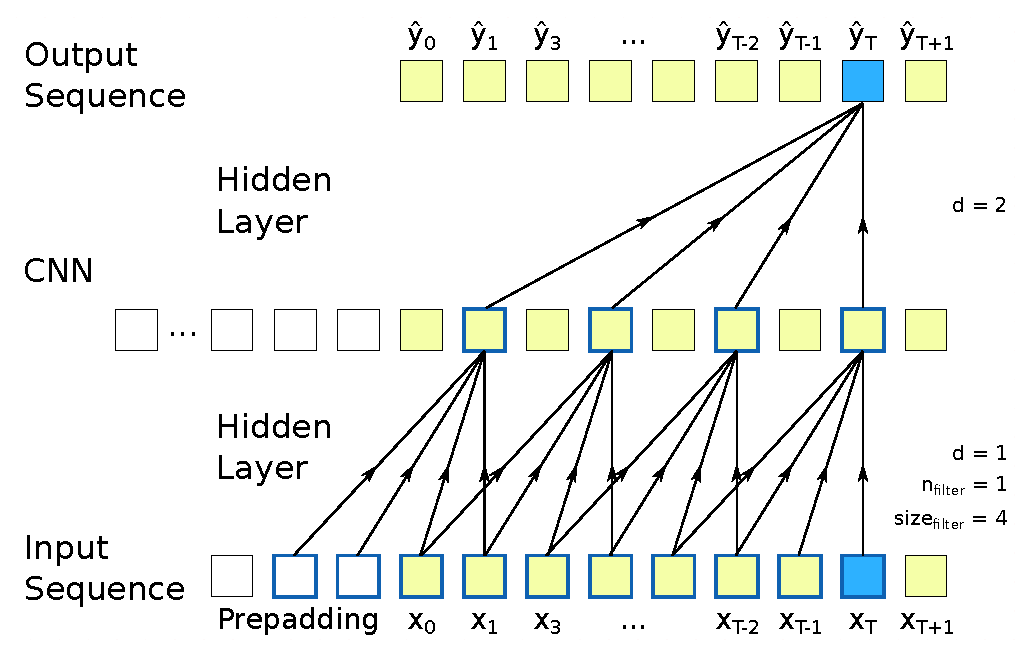
\includegraphics[width=0.75\textwidth]{modeling/CNN_over_sequence.eps}
    \caption{Convolutional Neural Network.}
	\label{fig:cnn}
\end{figure}

\section{Glossaries}
And this is not about \acrshort{CHP} or \gls{CHPg}

